% Dmitry Mikushin, USI Lugano, dmitry.mikushin@usi.ch,
% using portions of original style file by Tom Cashman
%
% IMPORTANT NOTICE:
%
% The USI logo is unique; it is authorized for use only by employees of the
% Università della Svizzera italiana for work-related projects; others can use them
% ONLY with prior authorization (contact: press@usi.ch).
%
% http://www.press.usi.ch/en/corporate-design/corporate-design-stampa.htm
%
% This is an example beamer presentation, which uses Università della Svizzera italiana
% design theme.

\documentclass[aspectratio=169]{beamer}

\usetheme{usi}
\usepackage{multirow}
\usepackage{hhline}
\usepackage{tikz}
\usepackage{graphicx}
\usepackage{caption}
\usepackage{subcaption}
\usepackage{listings}
\usepackage{array}
\usepackage{xcolor}
\usepackage{float}
\usetikzlibrary{shapes.geometric}

\newcommand\score[2]{
\pgfmathsetmacro\pgfxa{#1+1}
\tikzstyle{scorestars}=[star, star points=5, star point ratio=2.25, draw,inner sep=1.3pt,anchor=inner point 3]
  \begin{tikzpicture}[baseline]
    \foreach \i in {1,...,#2} {
    \pgfmathparse{(\i<=#1?"usi@yellow":"gray")}
    \edef\starcolor{\pgfmathresult}
    \draw (\i*2.0ex,0) node[name=star\i,scorestars,fill=\starcolor,color=\starcolor]  {};
   }
  \end{tikzpicture}
}

\definecolor{cadmiumgreen}{rgb}{0.0, 0.42, 0.24}

\setlength{\fboxsep}{0.25pt}%
\setlength{\fboxrule}{0pt}%

\title[Particle Simulations with OpenACC]{\textbf{Particle Simulations with OpenACC: Speedup and Scaling}\\[0.5em] Overview of mathematical models, simulation used, and OpenACC}
\author{Samuel A. Cruz Alegr\'{i}a, Alessandra M. de Felice, Hrishikesh R. Gupta}
\institute{(University of Lugano)}
\date{\today}


\begin{document}
\begin{frame}
\titlepage
\end{frame}
%-------------------------------------------------------------------------------
%-------------------------------------------------------------------------------

\begin{frame}[fragile]{Motivation \& Goals}

\begin{itemize}
\item Particle Simulations are essential for visualization of behaviour of physical systems 
\begin{itemize}
\item Molecular Dynamics
\item Celestial body simulations
\item Fluid dynamics 
\end{itemize}
\item Realistic computations have massive particle numbers and therefore immense computational costs
\item Multi-core simulation tools are essential for runtime optimization
\item Therefore our \textbf{goal} is to optimize particle simulation runtime using OpenACC parallelization and to observe scaling with an increasing number of particles.
\end{itemize}


\end{frame}
%-------------------------------------------------------------------------------
%-------------------------------------------------------------------------------
\begin{frame}[fragile]{Mathematical Models}
Molecular dynamics \emph{simulations} consist of the \emph{numerical} step-by-step solution of the classical equations of motion. For a simple atomic system, they may be written as follows:
%
\begin{equation}
	\begin{split}
	m_i \cdot \ddot{\*r_i} &= \*f_i, i = 1,...,N,\\
	f_i &= -\frac{\partial E_p}{\partial \*r_i},
	\end{split}
\end{equation}
%
where
%
\begin{itemize}
	\item $N$ is the number of atoms.
	\item $E_p(\*r^N)$ represents the potential energy.
	\item $\*r^N = (\*r_1, \*r_2, ..., \*r_n)$ represent the $3 \cdot n$ \emph{atomic coordinates}.
\end{itemize}
%

\end{frame}
%-------------------------------------------------------------------------------

%-------------------------------------------------------------------------------
\begin{frame}[fragile]{Force Fields}
In biochemical systems, commonly-used force fields model the \emph{potential energy} function as the sum of bonded, van der Waals, and electrostatic (Coulomb) energy:
%
\begin{equation}
	\label{eq:total_energy}
	E_p = E_{\text{bonded}} + E_{\text{non-bonded}}.
\end{equation}
%
The potential is a function of the positions of \emph{all} the atoms in the simulation. The \emph{force} on an atom is the negative gradient of this potential at the position of the atom:
%
\begin{equation}
	f = -\nabla E_p.
\end{equation}
%

\end{frame}
%-------------------------------------------------------------------------------

%-------------------------------------------------------------------------------
\begin{frame}[fragile]{Total Energy}
We can view equation the constituents of equation (\ref{eq:total_energy}) as follows:
%
\begin{equation}
	E_{\text{bonded}} = E_{\text{str}} + E_{\text{bend}} + E_{\text{tor}}.
\end{equation}
%
%
\begin{equation}
	E_{\text{non-bonded}} = E_{\text{Coul}} + E_{\text{vdW}}.
\end{equation}
%

The bonded interactions are named as such because the atoms involved must be directly bonded or bonded to a common atom.

\end{frame}
%-------------------------------------------------------------------------------

%-------------------------------------------------------------------------------
\begin{frame}[fragile]{Bonded Interactions}
We can model the bonded energy as follows:
%
\begin{equation}
	E_{\text{bonded}} = E_{\text{str}} + E_{\text{bend}} + E_{\text{tor}},
\end{equation}
%
where
%
\begin{itemize}
	\item $E_{\text{str}}$ is the energy required to \emph{stretch} or compress a given bond.
	\item $E_{\text{bend}}$ is the energy required to \emph{bend} a bond from its equilibrium angle, $\theta_{eq}$.
	\item $E_{\text{tor}}$ is the energy of \emph{torsion} needed to rotate about bonds. These are most relevant in single bonds because double and triple bonds are too rigid to permit rotation.
\end{itemize}
%

\end{frame}
%-------------------------------------------------------------------------------

%-------------------------------------------------------------------------------
\begin{frame}[fragile]{Stretch/Compression Energy}
A bond can be thought of as a spring having its own equilibrium length, $r_{eq}$, and the energy required to stretch or compress it can be approximated by the Hookian potential for an ideal spring:
%
\begin{equation}
	E_{\text{str}} = \frac{1}{2} \sum_{\text{bonds}} k_{ij}^s \left(r_{ij} - r_{\text{eq}}\right)^2,
\end{equation}
%
%
\begin{columns}
\begin{column}{0.5\textwidth}
	where
	%
	\begin{itemize}
		\item $k_{ij}^s$ is the stretching force constant for the bond.
		\item $r_{ij}$ is the distance between atoms $i$ and $j$.
	\end{itemize}
	%
\end{column}
%
\begin{column}{0.5\textwidth} 
	%
	\begin{figure}
		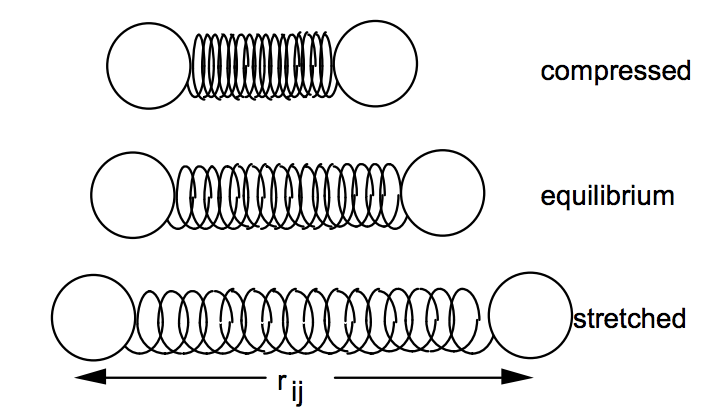
\includegraphics[scale=0.5]{Graphics/stretch.png}
		\caption{Bond Stretching.}
	\end{figure}
	%
\end{column}
\end{columns}
%

\end{frame}
%-------------------------------------------------------------------------------

%-------------------------------------------------------------------------------
\begin{frame}[fragile]{Bending Energy}
	
$E_{\text{bend}}$ is the energy required to \emph{bend} a bond from its equilibrium angle, $\theta_{eq}$. Once more, this system can be modeled by a spring, and the energy is given by the Hookian potential with respect to the angle:
%
\begin{equation}
	E_{\text{bend}} = \frac{1}{2} \sum_{\text{bend angles}} k_{ijk}^{b} \left(\theta_{ijk} - \theta_{eq} \right),
\end{equation}
%
%
\begin{columns}
\begin{column}{0.5\textwidth}
	where
	%
	\begin{itemize}
		\item $k_{ijk}^{b}$ is the bending force constant.
		\item $\theta_{ijk}$ is the instantaneous bond angle.
	\end{itemize}
	%
\end{column}
%
\begin{column}{0.5\textwidth} 
	%
	\begin{figure}
		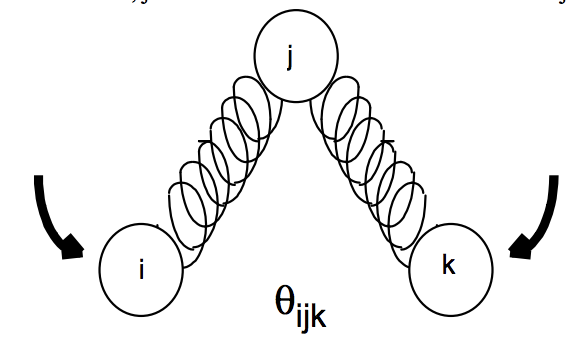
\includegraphics[scale=0.5]{Graphics/bend.png}
		\caption{Bond Bending.}
	\end{figure}
	%
\end{column}
\end{columns}
%

\end{frame}
%-------------------------------------------------------------------------------

%-------------------------------------------------------------------------------
\begin{frame}[fragile]{Torsion Energy}
	
$E_{\text{tor}}$ is the energy of \emph{torsion} needed to rotate about bonds. Torsional interactions can be modeled by the following potential:
%
\begin{equation}
	E_{\text{tor}} = \frac{1}{2} \sum_{\text{torsion angles}} \left( k_{tor,1}(1 + \cos \phi) + k_{tor,2}(1 + \cos 2\phi) + k_{tor,3}(1 + \cos 3\phi)\right),
\end{equation}
%
%
\begin{columns}
\begin{column}{0.5\textwidth}
	where
	%
	\begin{itemize}
		\item The angle $\phi$ is the dihedral angle about the bond.
		\item The constants $k_{tor,1}, k_{tor,2}, k_{tor,3}$ are the torsional constants for one-fold, two-fold, and three-fold rotational barriers, respectively. 
	\end{itemize}
	%
\end{column}
%
\begin{column}{0.5\textwidth} 
	%
	\begin{figure}
		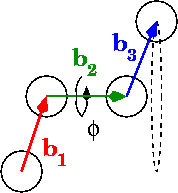
\includegraphics[scale=0.5]{Graphics/torsion.png}
		\caption{Bond Torsion.}
	\end{figure}
	%
\end{column}
\end{columns}
%

\end{frame}
%-------------------------------------------------------------------------------


%-------------------------------------------------------------------------------
\begin{frame}[fragile]{Bonded Interactions}
Putting it all together, we have the following for the bonded interactions:
%
\begin{equation}
\begin{split}
	E_{\text{bonded}} &= \frac{1}{2} \sum_{\text{bonds}} k_{ij}^s \left(r_{ij} - r_{\text{eq}}\right)^2 \\
	&+ \frac{1}{2} \sum_{\text{bend angles}} k_{ijk}^{b} \left(\theta_{ijk} - \theta_{eq} \right)\\
	&+ \frac{1}{2} \sum_{\text{torsion angles}} \left( k_{tor,1}(1 + \cos \phi) + k_{tor, 2}(1 + \cos 2\phi) + k_{tor, 3}(1 + \cos 3\phi)\right),
\end{split}
\end{equation}
%

\end{frame}
%-------------------------------------------------------------------------------

%-------------------------------------------------------------------------------
\begin{frame}[fragile]{Non-Bonded Interactions}
We can model the non-bonded energy as follows:
%
\begin{equation}
	E_{\text{non-bonded}} = E_{\text{Coul}} + E_{\text{vdW}},
\end{equation}
%
where
%
\begin{itemize}
	\item $E_{\text{Coul}}$ is the electrostatic energy resulting from charged molecules.
	\item $E_{\text{vdW}}$ is the energy resulting from the attraction of intermolecular forces, i.e., between molecules.
\end{itemize}
%

\end{frame}
%-------------------------------------------------------------------------------

%-------------------------------------------------------------------------------
\begin{frame}[fragile]{Non-Bonded Interactions}

In order to model the \emph{van der Waals forces}, we can use the Lennard-Jones function:
%
\begin{equation}
	E_{\text{vdW}} = \sum_{i=1}^{N-1} \sum_{j > i} 4\epsilon_{ij} \left[\left(\frac{\sigma_{ij}}{r_{ij}}\right)^{12} - \left(\frac{\sigma_{ij}}{r_{ij}}\right)^6 \right],
\end{equation}
%
%
\begin{columns}
\begin{column}{0.5\textwidth}
	where
	%
	\begin{itemize}
		\item $r_{ij}$ is the \emph{distance} between atoms $i$ and $j$.
		\item $\sigma_{ij}$ is the finite distance at which inter-particle potential is zero.
		\item $\epsilon_{ij}$ is the depth of the potential well, which is a region surrounding a local minimum of potential energy.
	\end{itemize}
	%
\end{column}
%
\begin{column}{0.5\textwidth} 
	%
	\begin{figure}
		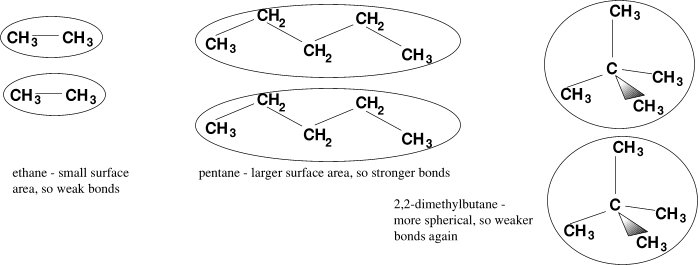
\includegraphics[scale=0.3]{Graphics/vdW.png}
		\caption{van der Waals Forces.}
	\end{figure}
	%
\end{column}
\end{columns}
%

\end{frame}
%-------------------------------------------------------------------------------

%-------------------------------------------------------------------------------
\begin{frame}[fragile]{Non-Bonded Interactions}

If charges are present, we can model the electrostatic energy due to the atomic charges using the Coulombic potential function:
%
\begin{equation}
	E_{\text{Coul}} = \sum_{i=1}^{N-1} \sum_{j>i} \frac{q_i q_j}{4\pi\epsilon_0r_{ij}},
\end{equation}
%
%
\begin{columns}
\begin{column}{0.5\textwidth}
	where
	%
	\begin{itemize}
		\item $r_{ij}$ is the distance between atoms $i$ and $j$.
		\item $q_i$ and $q_j$ are the charges of atoms $i$ and $j$, respectively.
		\item $\epsilon_0 \approx 8.85 × 10^{-12} m^{-3} kg^{-1} s^4 A^2$ (permittivity of free space).
	\end{itemize}
	%
\end{column}
%
\begin{column}{0.5\textwidth} 
	%
	\begin{figure}
		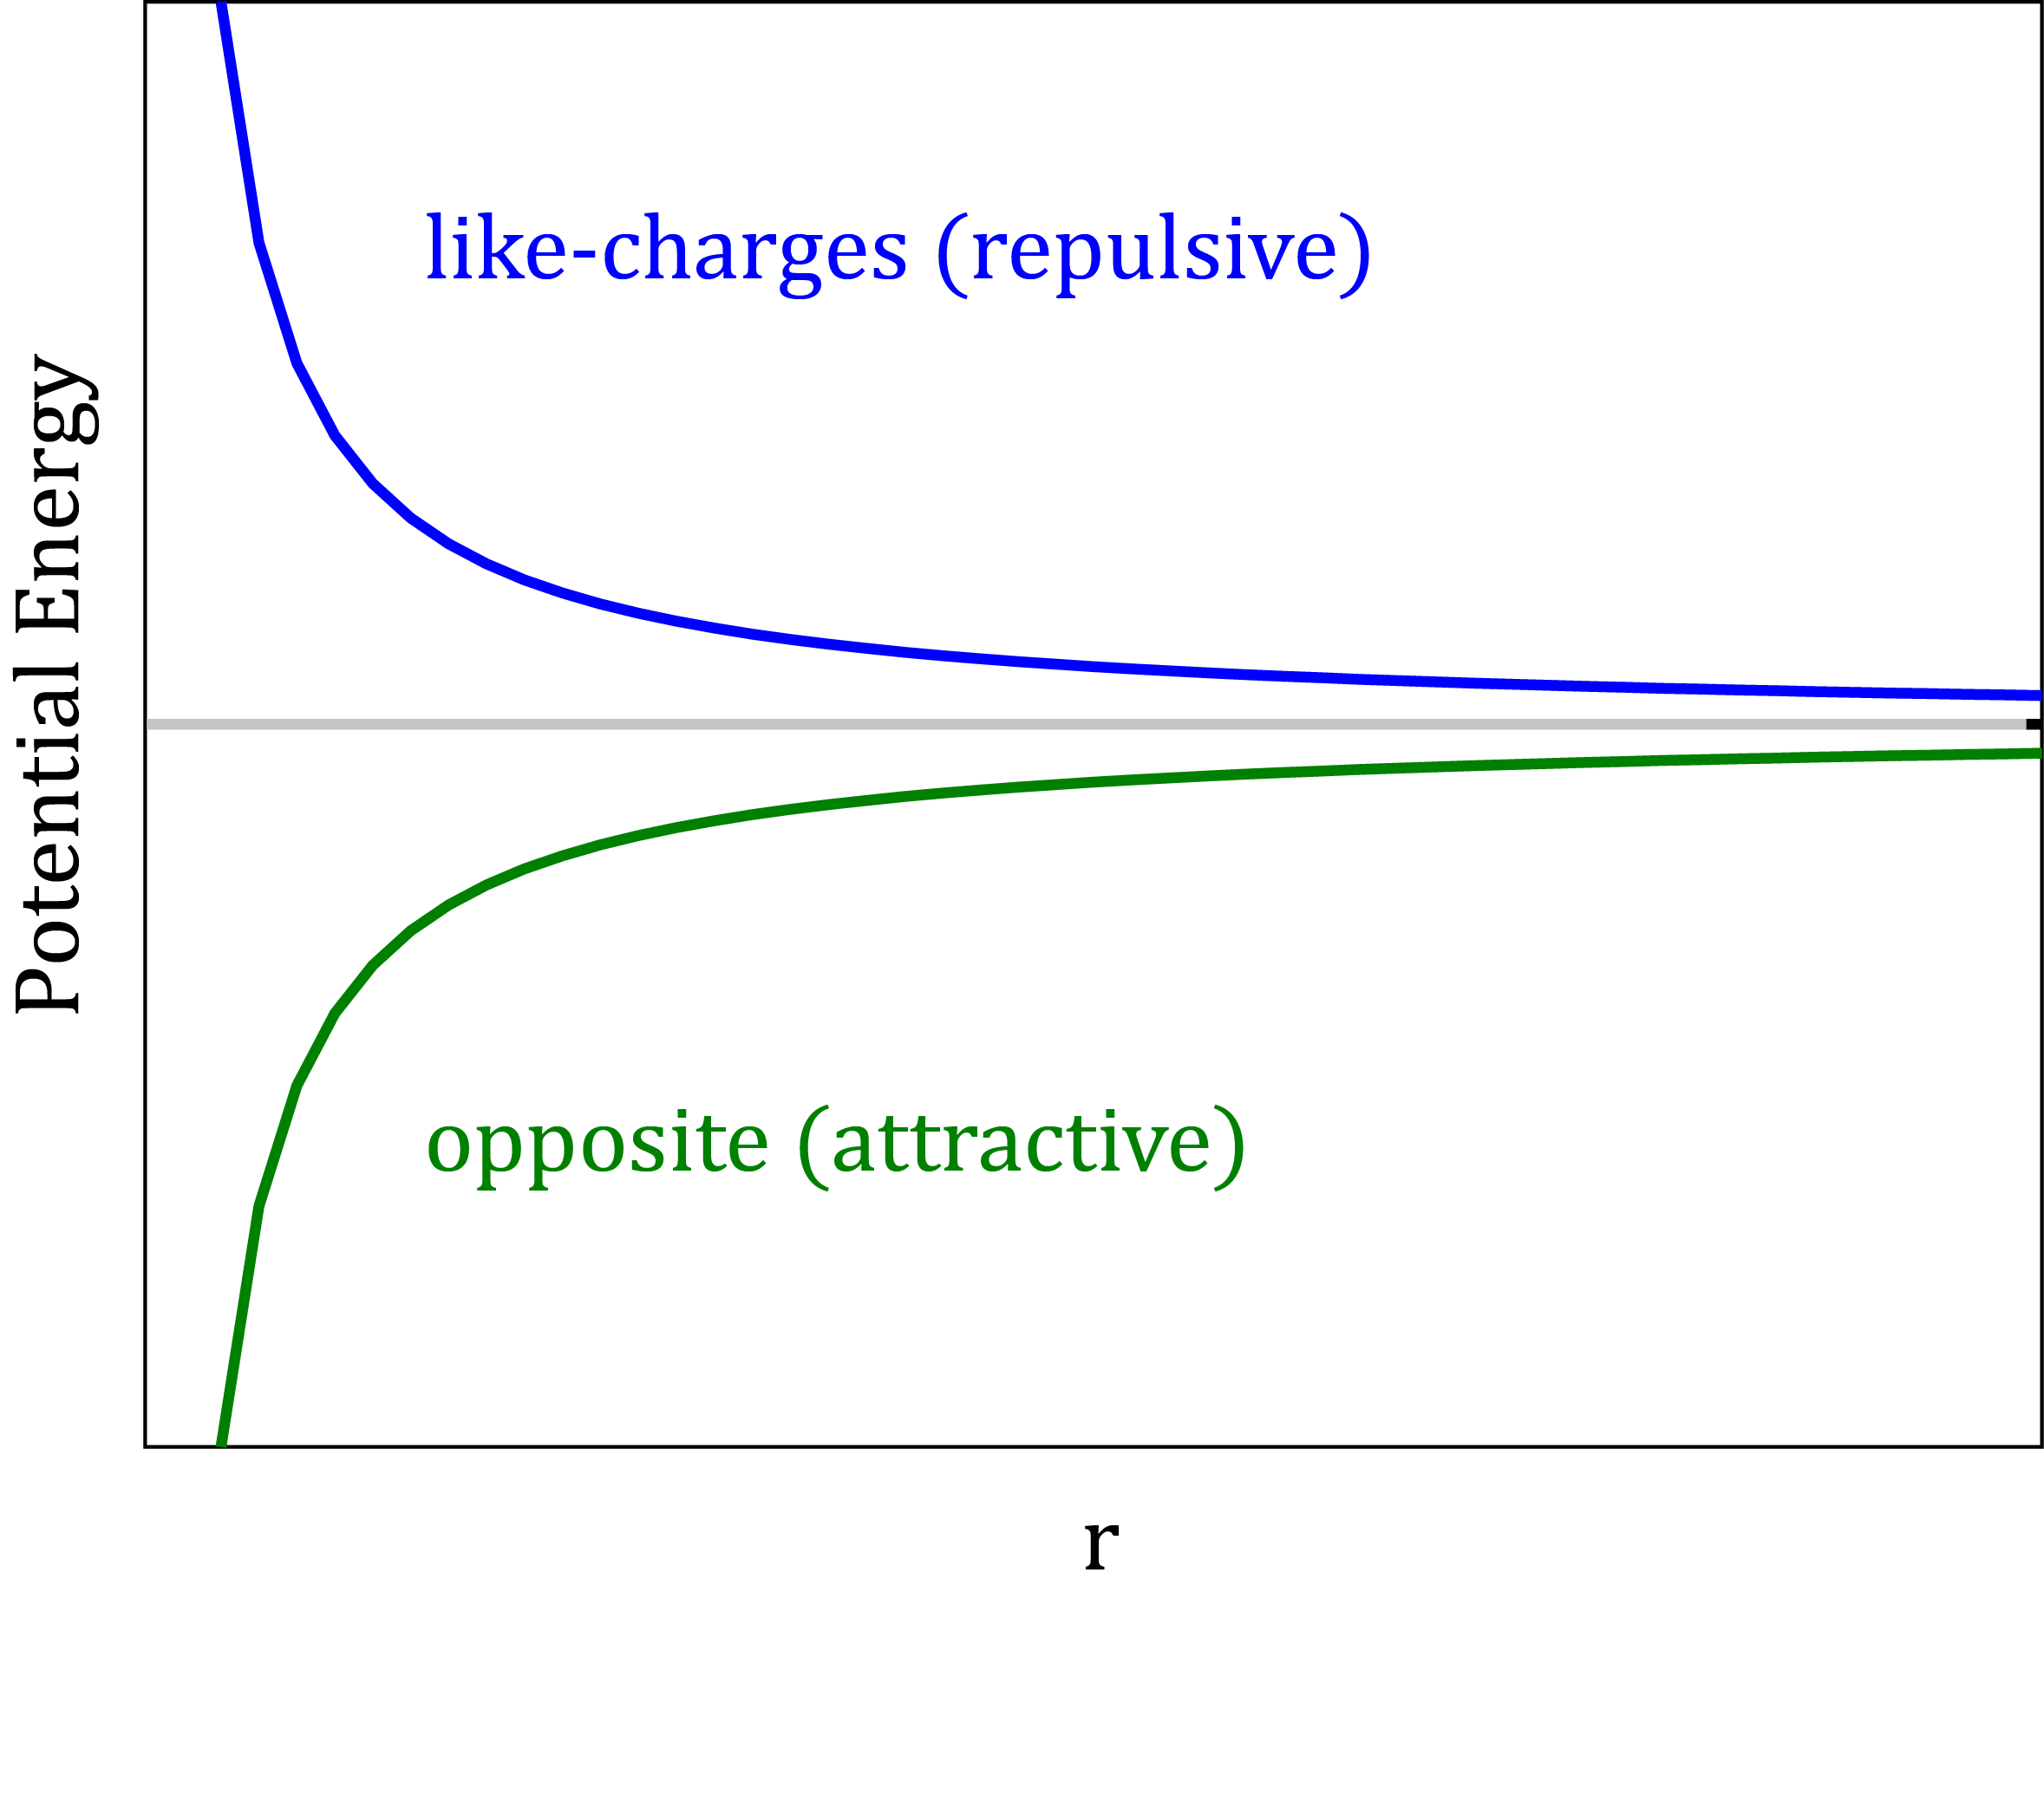
\includegraphics[scale=0.225]{Graphics/coulomb.png}
		\caption{Coulomb Potential.}
	\end{figure}
	%
\end{column}
\end{columns}
%

\end{frame}
%-------------------------------------------------------------------------------

%-------------------------------------------------------------------------------
\begin{frame}[fragile]{Updating Position}

Once more, once we have computed the potential energy, we can compute the force on an atom as the negative gradient of this potential at the position of the atom:
%
\begin{equation}
	f_i = -\frac{\partial E_p}{\partial \*r_i},
\end{equation}
%
and we can then proceed to update the position of the atom based on a given algorithm, such as $r_i^{k+1} = r_i^{k} + 0.5 \cdot \Delta t \cdot f$.

\end{frame}
%-------------------------------------------------------------------------------



%-------------------------------------------------------------------------------

\begin{frame}[fragile]{Simulation}

\begin{itemize}
\item \textbf{Idea}
\begin{itemize}
\item Given, initial positions, masses and other parameters (Forces) for the particles future trajectory can be computed numerically for each particle.
\item Time step is thus composed of two parts:
\begin{itemize}
\item Compute forces on all particles
\item Update positions
\end{itemize}
\end{itemize}
\end{itemize}


\end{frame}
%-------------------------------------------------------------------------------
%-------------------------------------------------------------------------------
%-------------------------------------------------------------------------------

\begin{frame}[fragile]{Force Field}

\begin{itemize}
\item It is the model of potential energy and forces that acts between particles.
\item Commonly used force fields model the potential energy function as the sum of:
\begin{equation}
E_p = E_{bonded}+E_{Coul}+E_{VdW}
\end{equation}
\item Which is summation of Bonded Energy, Electrostatic Energy and Van der Waals Energy.
\end{itemize}



\end{frame}
%-------------------------------------------------------------------------------%-------------------------------------------------------------------------------

\begin{frame}[fragile]{Computing the forces (Short Range)}


\begin{itemize}
\item Mostly for non-bonded forces: electrostatic interactions and Van der Waals interactions.
\item Naïve approach:
\begin{itemize}
\item Examine all other particles and compute their distance to particle ‘i’. 
\item For ‘n’ particles, the complexity of this approach is O($n^2$), which is equivalent to computing forces between all pairs of particles. 
\end{itemize}
\item Cell Lists:
\begin{itemize}
\item Particle space is put in a grid.
\item The forces is computed on particle ’i’ in a grid cell with respect to 8 adjacent cells.
\item Complexity is O(n x average no. of particles in 9 cells).
\end{itemize}
\end{itemize}



\end{frame}
%-------------------------------------------------------------------------------%-------------------------------------------------------------------------------

\begin{frame}[fragile]{Computing the forces (Long Range)}
\begin{columns}
\column{0.5\textwidth}

\begin{itemize}
\item In order to avoid complexity O($n^2$) using naïve approach, following are some accurate methods.
\item \textbf{Particle Mesh Method:}
\begin{itemize}
\item A system of particles, converted into mesh or grid values.
\item we exploit the Poisson equation:
\begin{equation}
\triangledown^2\phi = - \frac{1}{\epsilon}\rho
\end{equation}
\item Relates potential $\phi$ to charge density $\rho$, where $\frac{1}{\epsilon}$ is a constant.
\item Charges are assigned to mesh point and equation (16) is solved to arrive at the potential on the mesh.
\end{itemize}
\end{itemize}

\column{0.5\textwidth}
\begin{itemize}
\item The force is the negative gradient of the potential.
\item Fast methods such as multi-grid method and FFT are used to solve Poisson’s equation.
\end{itemize}
\begin{itemize}
\item \textbf{Ewald Method:}
\begin{itemize}
\item The force is split between short-range and long-range.
\item Short-range part is computed using particle-particle methods.
\item Long-range part is computed using Fourier Transforms.
\end{itemize}
\end{itemize}
\end{columns}
\end{frame}
%-------------------------------------------------------------------------------
%-------------------------------------------------------------------------------

\begin{frame}[fragile]{Parallel Approaches}


\begin{itemize}
\item \textbf{Atom Decomposition:}
\begin{itemize}
\item Each particle is assigned to one processor, which is responsible for computing the particle’s forces and updating its position for the entire simulation.
\item Each processor communicates with all other processors to share updated particle positions.
\item An Force-matrix is constructed, which is an n-by-n matrix; the rows and columns are numbered by particle indices. 
\item Each point in force-matrix computes, force on ‘i’ due to particle ‘j’.
\item When cutoffs are used, the matrix is sparse.
\end{itemize}
\begin{figure}
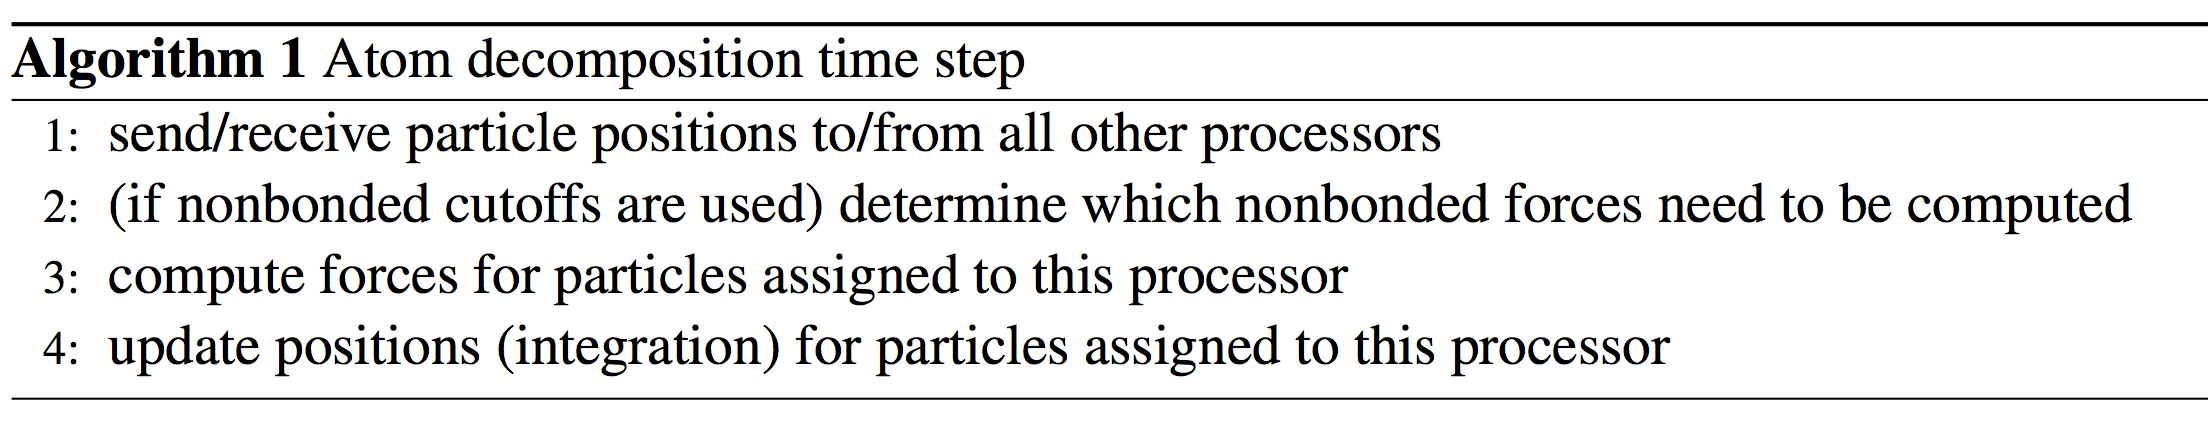
\includegraphics[scale=0.3]{Graphics/slide_6.png}
\end{figure}
\end{itemize}


\end{frame}
%-------------------------------------------------------------------------------
%-------------------------------------------------------------------------------

\begin{frame}[fragile]{Parallel Approaches}


\begin{itemize}
\item \textbf{Spatial Decomposition}
\begin{itemize}
\item Space is divided into cells and each cell is assigned to a processor, responsible for computing the forces on particles that lie inside the cell. 
\item Since particles move during the simulation, the assignment of particles to cells changes as well. 
\item Cutoff radius decides import region and the given cell must import positions of particles lying in this region to perform its force calculation. 
\begin{figure}
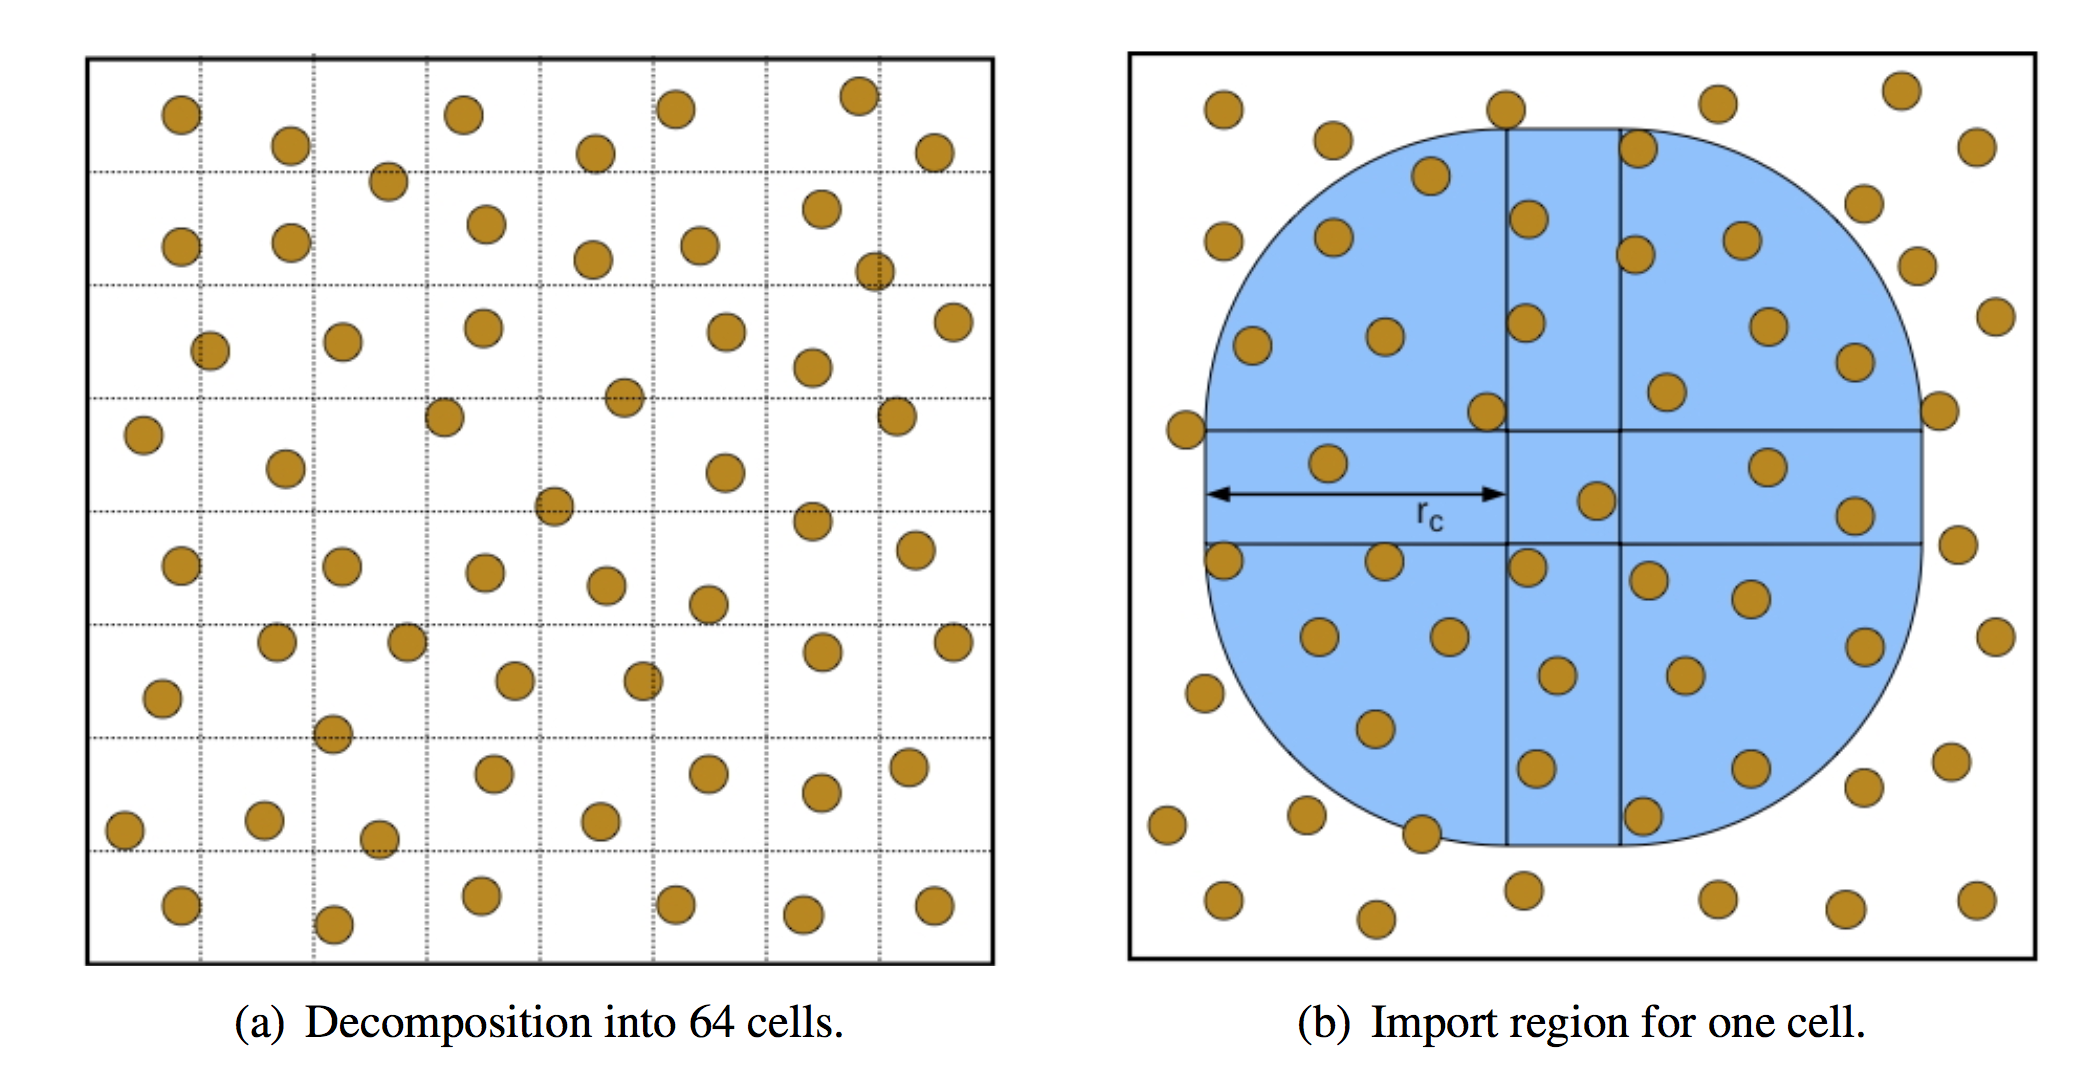
\includegraphics[scale=0.2]{Graphics/slide_7.png}
\end{figure}
\end{itemize}
\end{itemize}



\end{frame}
%-------------------------------------------------------------------------------
%-------------------------------------------------------------------------------

\begin{frame}[fragile]{Parallel Approaches}


\begin{itemize}
\item \textbf{Neutral Territory Method:}
\begin{itemize}
\item Particles are assigned to processors according to a partitioning of space.
\item Each processor computes the forces between two sets of particles, these particles may be unrelated to the particles that have been assigned to the processor.
\item For example: The given processor is assigned the computation of forces between particles lying in the horizontal bar with particles lying in the vertical bar. 
\end{itemize}
\begin{figure}
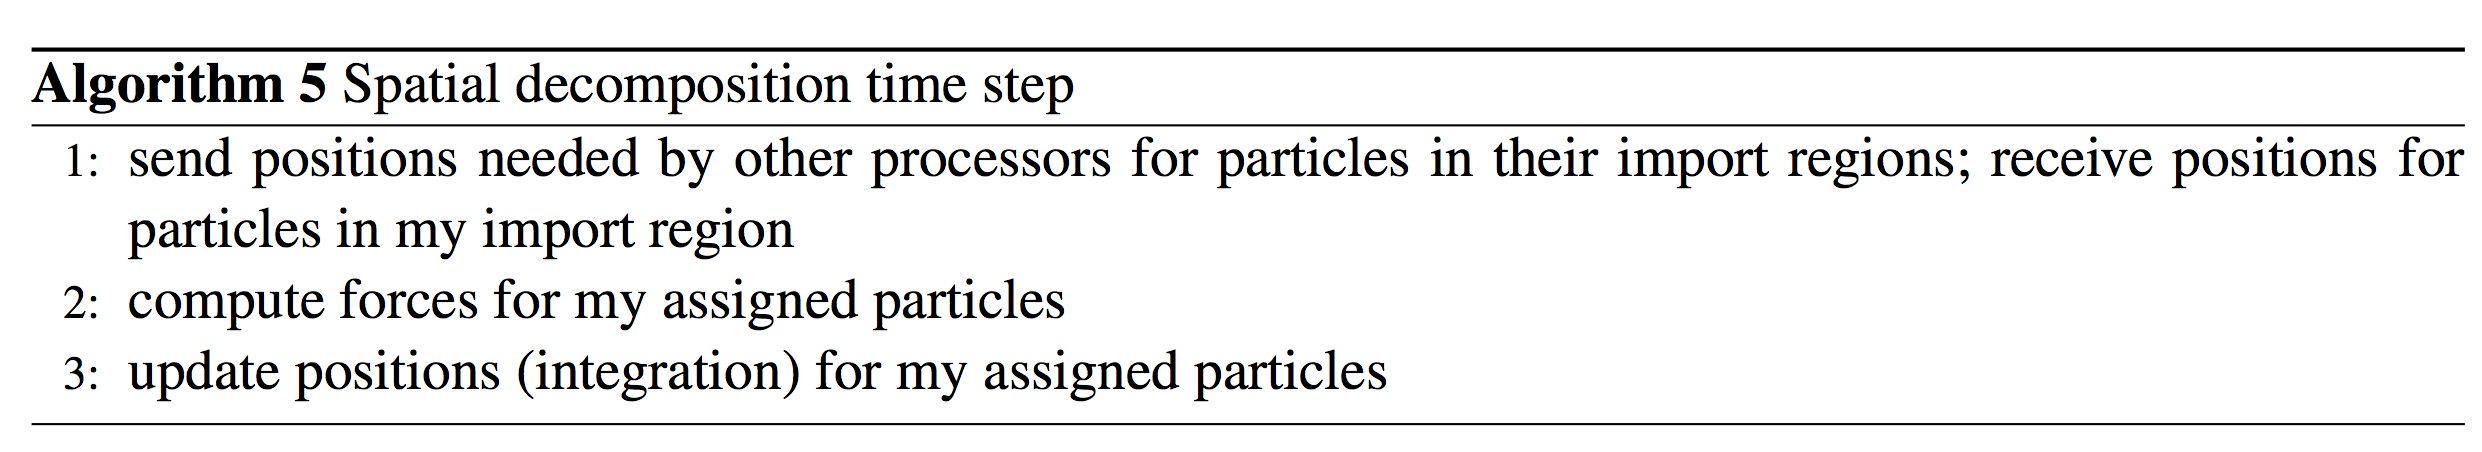
\includegraphics[scale=0.3]{Graphics/slide_8.png}
\end{figure}
\end{itemize}


\end{frame}
%-------------------------------------------------------------------------------
%-------------------------------------------------------------------------------

\begin{frame}[fragile]{Parallel Approaches}


\begin{itemize}
\item These two regions thus form the import region.
\begin{figure}[H]
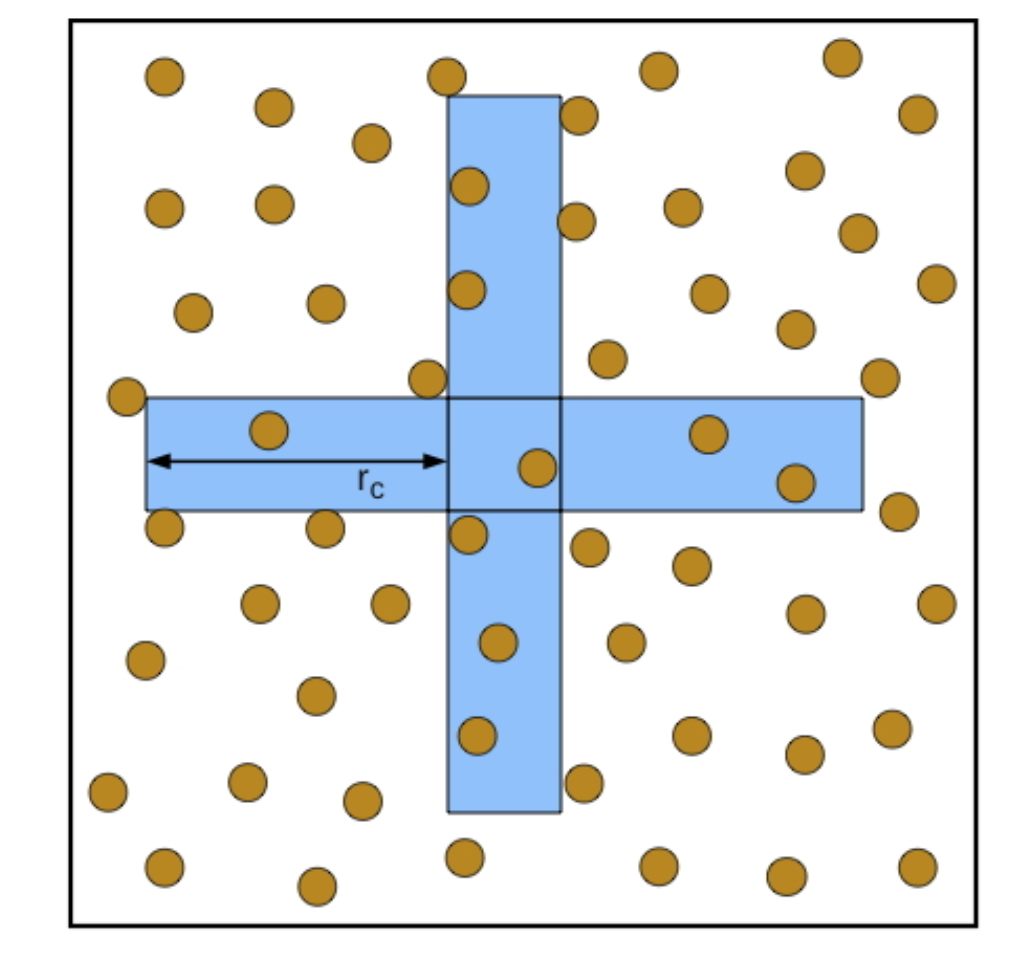
\includegraphics[scale=0.2]{Graphics/slide_9.png}
\end{figure}
\item After the forces are computed, the given processor sends the forces it has computed to the processors that need these forces for integration. 

\end{itemize}



\end{frame}
%-------------------------------------------------------------------------------
%-------------------------------------------------------------------------------

\begin{frame}[fragile]{OpenACC}
\centering\textbf{"The execution of CUDA with the simplicity of OpenMP"}\bigskip

\begin{itemize}
\item \textbf{What is OpenACC?}
	\begin{itemize}
	\item Accelerator based parallel programming
    \item Like OpenMP, OpenACC uses directive based programming
    \begin{itemize}
    \item Compiler generates the parallel code
    \end{itemize}
	\item Used with C/C++ and Fortan
    \item OpenACC uses GPU (or multicore CPU) acceleration incrementally
	\end{itemize}
\end{itemize}


\end{frame}
%-------------------------------------------------------------------------------
%-------------------------------------------------------------------------------

\begin{frame}[fragile]{OpenACC}
\begin{columns}
\column{0.5\textwidth}
\begin{itemize}
\item \textbf{Advantages}
	\begin{itemize}
	\item High level
    \begin{itemize}
    \item The compiler will ultimately make the decision as to where this memory will be allocated and how it is addressed
    \item Programmer only deals with abstractions of memory and not memory itself
    \end{itemize}
    \item Performance portable
    \item Single source - No forking off a separate GPU code
    \item Efficient -  favorable comparison to low-level implementations of same algorithms
	\end{itemize}
\end{itemize}

\column{0.5\textwidth}
\begin{itemize}
\item Incremental - can port and tune parts of their application as resources and profiling dictates.
 \begin{itemize}
    \item This is the disadvantage of CUDA
    \end{itemize}
    \item Implicit use of accelerators
   
\end{itemize}
 
\begin{itemize}
\item \textbf{Disadvantages}
\begin{itemize}
\item Some cases performance is 50\% lower than  CUDA implemented parallelization 
\item Complexity of implementation increases with complexity of loops
\begin{itemize}
\item This means that the time-saving advantage may be negated
\end{itemize}
\item Lack of a programming interface for the shared memory
\end{itemize}
\end{itemize}

\end{columns}
\end{frame}
%-------------------------------------------------------------------------------
%-------------------------------------------------------------------------------

\begin{frame}[fragile]{Where is OpenACC used?}

\begin{itemize}
\item Matrix Matrix Multiplication - 4 directives = 16x faster
\item Derivative Valuation - Few hours = 70x faster
\item N-body/Particle Simulations = 1 week = 3x faster
\item Real-time Image extraction - 3 directives = 4.1x faster
\item Fluid Dynamics and Fuel Combustion  = 4x Faster with less than 1\% of code modified
\item DNA sequence Analysis - 4 directives = 16x faster
\item Designing circuits for quantum
computing = 1 week = 40x faster
\end{itemize}

\end{frame}
%-------------------------------------------------------------------------------
%-------------------------------------------------------------------------------

\begin{frame}[fragile]{GPU Acceleration}
\begin{columns}
\column{0.5\textwidth}

\begin{itemize}
\item GPU vs CPU performance
\begin{itemize}
\item CPU consists of a few cores optimized for sequential serial processing
\item GPU has a massively parallel architecture consisting of thousands of smaller, more efficient cores designed for handling multiple tasks simultaneously.
\item GPU-accelerated computing offloads compute-intensive portions of the application to the GPU
\item Remainder of the code still runs on the CPU. 
\end{itemize}
\end{itemize}

\column{0.5\textwidth}
\begin{figure}
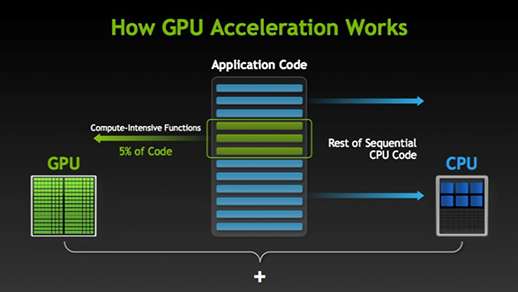
\includegraphics[scale=0.4]{Graphics/GPU.png}
\end{figure}
\end{columns}
\end{frame}
%---------------------------------------
%-------------------------------------------------------------------------------
%-------------------------------------------------------------------------------

\begin{frame}[fragile]{How OpenACC works?}
\begin{columns}
\column{0.5\textwidth}
\begin{figure}
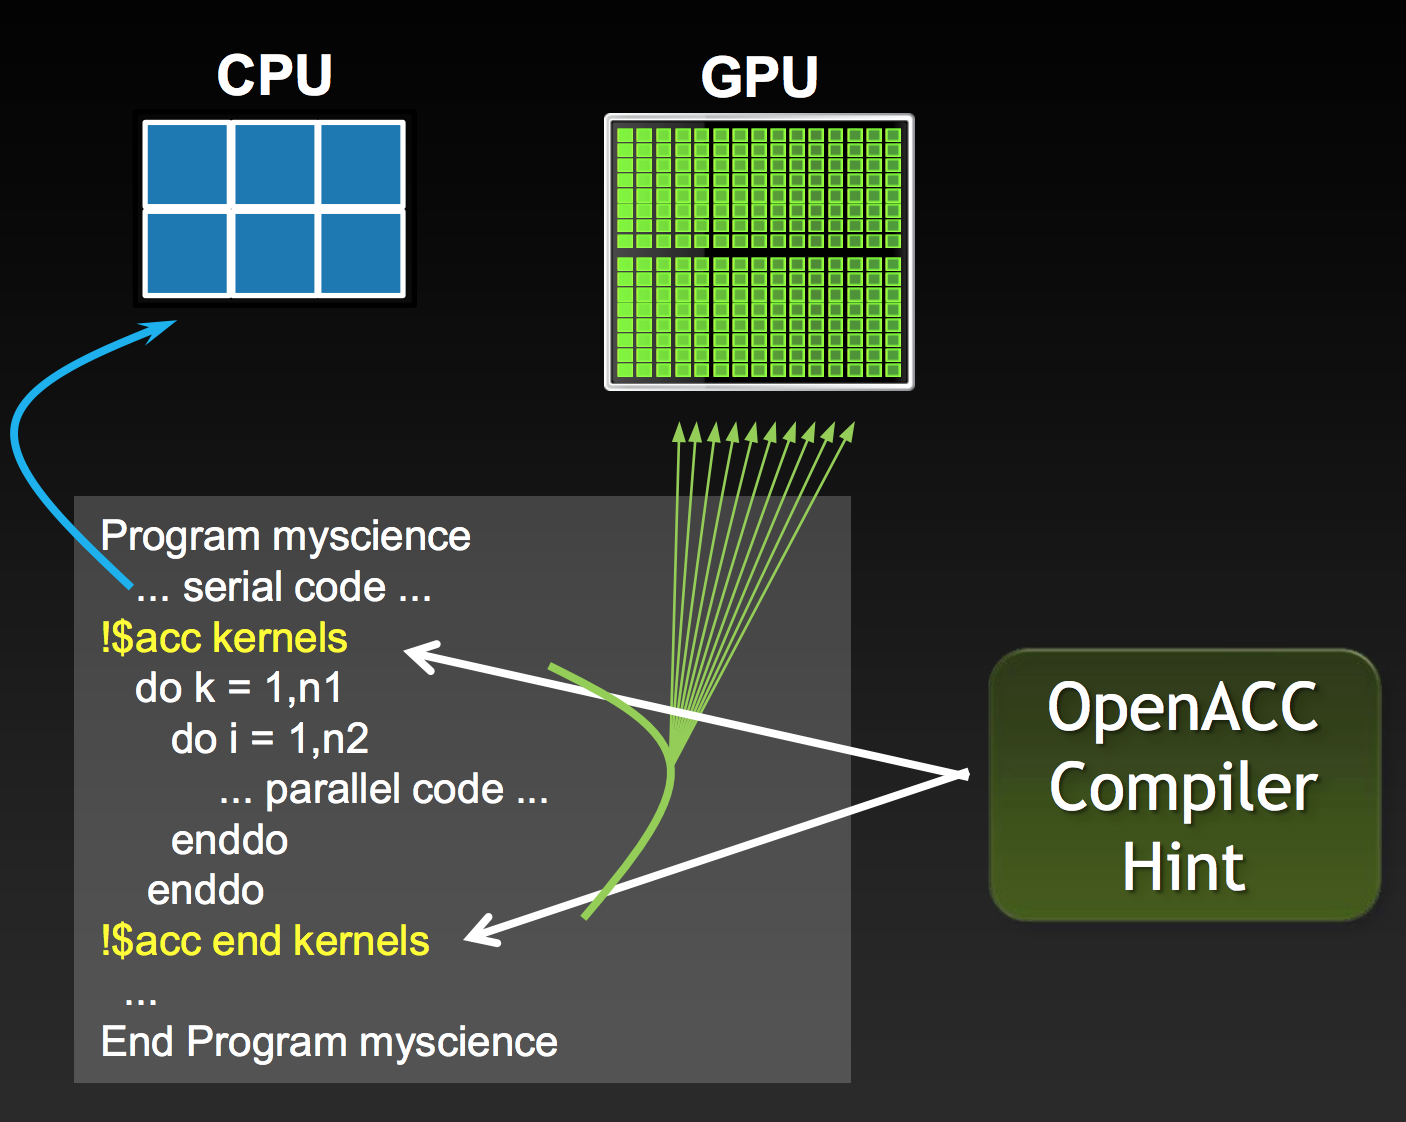
\includegraphics[scale=0.3]{Graphics/How.png}
\end{figure}
\column{0.5\textwidth}

\begin{itemize}
\item Parallelizeable code is moved from the host CPU to an accelerator device (GPU) for execution
\item Internal Control Variables (ICVs) - determine the type of accelerator device and which accelerator device
\item The environment variables (can be altered) → directive can be applied to certain accelerators or all accelerators 
\begin{itemize}
\item device type
\item device number
\end{itemize}
\end{itemize}

\end{columns}
\end{frame}
%-------------------------------------------------------------------------------

\begin{frame}[fragile]{Directives}

\begin{itemize}
\item \#pragma acc parallel loop directive
\begin{itemize}
\item Caution: the compiler will attempt to run the code in the for loop in parallel even if it is not safe to do so
\item This directive should be used with caution only when the underlying algorithm is completely understood
\end{itemize}
\item OpenACC kernel construct
\begin{itemize}
\item Make the code within the block parallel by creating accelerator kernels where possible and safe to do so.
\begin{itemize}
\item safe way to make your code parallel
\item Disadvantage = generated code may not always be the most efficient code possible. 
\end{itemize}
\item Kernels generated will run on the GPU
\end{itemize}
\end{itemize}



\end{frame}
%-------------------------------------------------------------------------------
%-------------------------------------------------------------------------------

\begin{frame}[fragile]{Performance comparison}
\begin{columns}
\column{0.5\textwidth}

\begin{itemize}
\item OpenACC and CUDA
\begin{itemize}
\item simple matrix computation - asked to compiler to run kernels on the device where possible
\end{itemize}

\item OpenACC and OpenMP
\begin{itemize}
\item computes the number of brights spots in a matrix that represents pixel brightness in an image.
\end{itemize}
\end{itemize}

\column{0.5\textwidth}
\begin{figure}
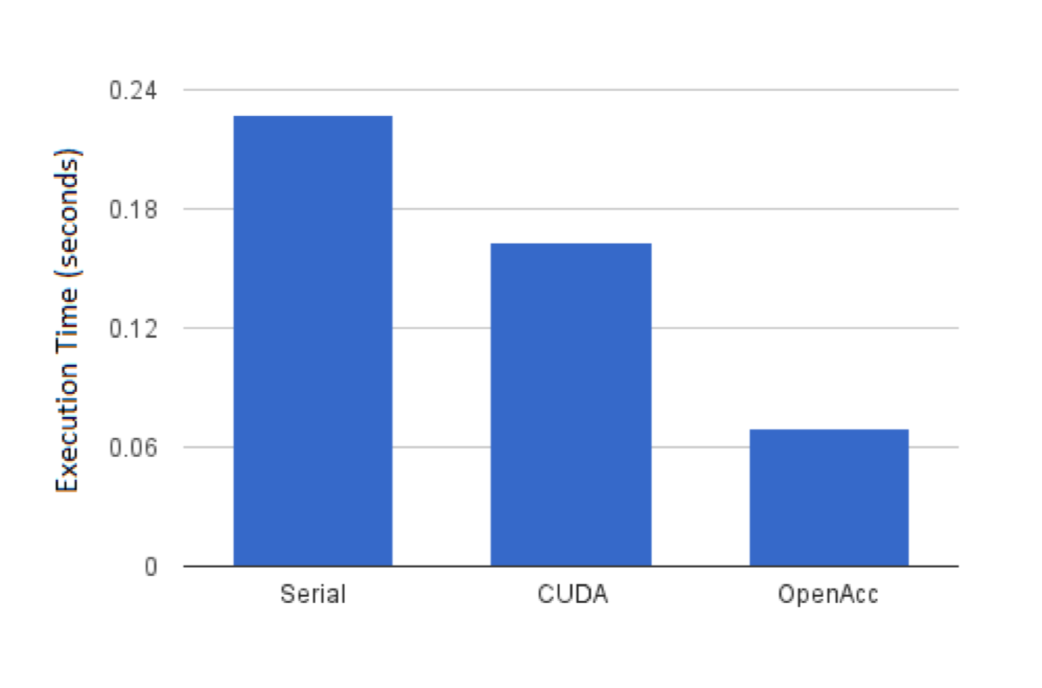
\includegraphics[scale=0.25]{Graphics/CUDA.png}
\end{figure}
\begin{figure}
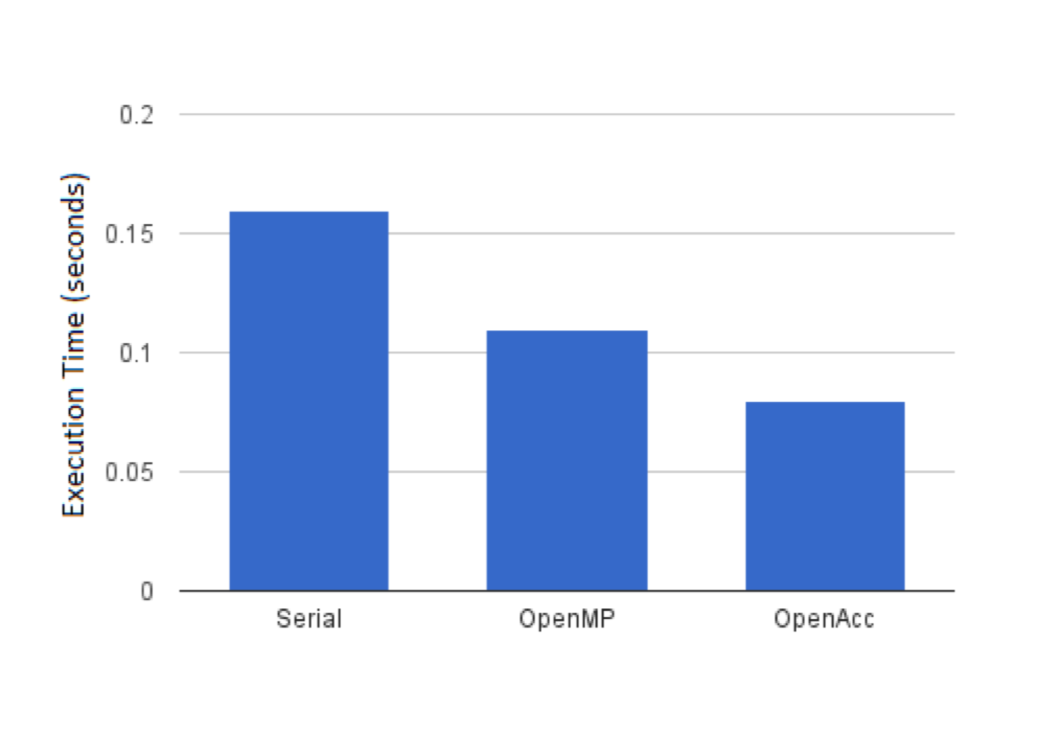
\includegraphics[scale=0.25]{Graphics/OMP.png}
\end{figure}
\end{columns}

\end{frame}
%-------------------------------------------------------------------------------
%-------------------------------------------------------------------------------%-------------------------------------------------------------------------------%-------------------------------------------------------------------------------

\begin{frame}[fragile]{Conclusion}

\begin{itemize}
\item In conclusion, N-body simulations are considered of great importance and it is thus essential to execute simulations as efficiently as possible.
\item Accelerator-based parallelization like OpenACC may prove to be a more efficient means to parallelize particle simulations because it is evident that this has not been explored thoroughly.
\end{itemize}



\end{frame}
%-------------------------------------------------------------------------------%-------------------------------------------------------------------------------



\begin{frame}[fragile]{References}

\begin{itemize}
\small{\item Farber, R., 2016.Parallel programming with OpenACC. Newnes.
\item Gonzales, R.,  Martin, M., Mittow, N., and Rasmuss, R.,2016, An Introduction to OpenAcc.ECS 158 Final Project.
\item Li, X., Shih, P.C., Overbey, J., Seals, C. and Lim, A., 2016. Comparing programmer productivity in OpenACC and CUDA: an empirical investigation.International Journal of Computer Science, Engineering and Applications (IJCSEA),6(5), pp.1-15.
\item Memeti, S., Li, L., Pllana, S., Kołodziej, J. and Kessler, C., 2017, July. Benchmarking OpenCL, OpenACC, OpenMP, and CUDA: programming productivity, performance, and energy consumption. InProceedings of the 2017 Workshop on Adaptive Resource Management and Scheduling for Cloud Computing(pp. 1-6). ACM.
\item Urbanic, J., 2013. Introduction to Directive Based Programming.
\item OpenACC Programming and Best Practices. Guide \url{http://www.openacc.org/sites/default/files/inline-files/OpenACC_Programming_Guide_0.pdf}
\item \url{http://www.nvidia.com/object/what-is-gpu-computing.html}}
\item Allen, M.P., 2004. Introduction to molecular dynamics simulation. Computational soft matter: from synthetic polymers to proteins, 23, pp.1-28.
\item Eijkhout, V., 2014. Introduction to High Performance Scientific Computing. Lulu. com.
\end{itemize}

\end{frame}
%-------------------------------------------------------------------------------

\end{document}
